% 使用ctexart文档类(用XeLaTeX编译,直接支持中文)
\documentclass[fleqn]{ctexart}

% 中文
%\usepackage{ctex}
% 平面几何绘图
\usepackage{tkz-euclide}
\usetkzobj{all}
\usepackage{amsthm}
\usepackage{amsmath}
\usepackage{txfonts}
\usepackage{floatrow}
\usepackage[hypcap=true]{caption}

% 取消默认的冒号
\captionsetup{labelsep=space}
% 居中
\floatsetup[figure]{objectset=centering}

\begin{document} %在document环境中撰写文档

已知:直线$AB\varparallel CD$,点$P$为平面上一点,连接$AP$与$CP$。

(1)如\ref{fig01},点$P$在直线$AB$、$CD$之间,当$\angle BAP=60^\circ$,
$\angle DCP=20^\circ$时,求$\angle APC$。

(2)如\ref{fig02},点$P$在直线$AB$、$CD$之间,当$\angle BAP$与$\angle
DCP$的角平分线相交于$K$,写出$\angle AKC$与$\angle APC$之间的数量关系,
并说明理由。

(3)如\ref{fig03},点$P$落在$CD$之外,$\angle BAP$与$\angle
DCP$的角平分线相交于$K$,$\angle AKC$与$\angle APC$有何数量关系?
并说明理由。

\begin{figure}[!htp]
  \begin{floatrow}
    \ffigbox[1.0\FBwidth]
    {
      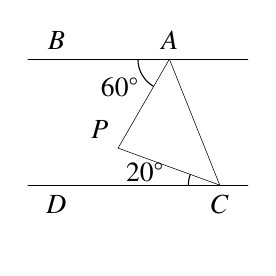
\begin{tikzpicture}[
        scale=0.8,
        decoration={
          markings,
          mark=at position 3cm with {\arrow[scale=2]{>}};
        }]
        % 初始化
        \tkzInit[xmin=-0.25,xmax=3.25, ymin=-1.00,ymax=2.5] \tkzClip
        % 定义坐标点
        \tkzDefPoints{0/0/E, 3/0/F, 0/2/R, 3/2/S}
        % 绘制两条平行线
        \tkzDrawLines(E,F R,S)
        % 定义A、B、C、D坐标
        \tkzDefPoints{0.2/0/D, 2.8/0/C, 0.2/2/B, 2.0/2/A}
        % 绘制各线段
        \tkzDrawSegments(A,C)
        % 标记符号
        \tkzLabelPoints[above](A,B)
        \tkzLabelPoints[below](D,C)
        % 定义A出发-120度的线
        \tkzDefShiftPoint[A](-120:1){a}
        % 定义C出发110度的线
        \tkzDefShiftPoint[C](160:1){c}
        % 求交点
        \tkzInterLL(A,a)(C,c) \tkzGetPoint{P}
        \tkzLabelPoints[above left](P)
        % %\tkzShowLine[parallel=through P](E,F)
        % \tkzDefLine[parallel = through P](E,F) \tkzGetPoint{p}        
        % \tkzDrawLines[color = red,add=.6 and .6,dashed](P,p)
        % 绘制线段
        \tkzDrawSegments(A,P C,P)   
        \tkzMarkAngle[fill=red,size=0.5](P,C,D)
        \tkzLabelAngle[pos=1.2](P,C,D){$20^\circ$}
        \tkzMarkAngle[fill=blue,size=0.5](B,A,P)
        \tkzLabelAngle[pos=-0.9](P,A,B){$60^\circ$}
      \end{tikzpicture}
    }{\caption{}\label{fig01}}
    \ffigbox[1.0\FBwidth]%[\Xhsize]
    {
      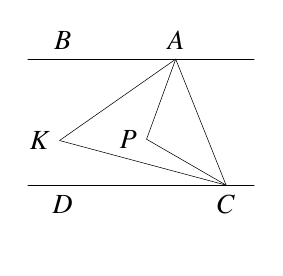
\begin{tikzpicture}[
        scale=0.8,
        decoration={
          markings,
          mark=at position 3cm with {\arrow[scale=2]{>}};
        }]
        % 初始化
        \tkzInit[xmin=-0.35,xmax=3.25, ymin=-1.0,ymax=2.5] \tkzClip
        % 定义坐标点
        \tkzDefPoints{0/0/E, 3/0/F, 0/2/R, 3/2/S}
        % 绘制两条平行线
        \tkzDrawLines(E,F R,S)
        % 定义A、B、C、D坐标
        \tkzDefPoints{0.2/0/D, 2.8/0/C, 0.2/2/B, 2.0/2/A}
        % 绘制各线段
        \tkzDrawSegments(A,C)
        % 标记符号
        \tkzLabelPoints[above](A,B)
        \tkzLabelPoints[below](D,C)
        % 定义A出发-120度的线
        \tkzDefShiftPoint[A](-110:1){a}
        % 定义C出发110度的线
        \tkzDefShiftPoint[C](150:1){c}
        % 求交点
        \tkzInterLL(A,a)(C,c) \tkzGetPoint{P}
        \tkzLabelPoints[left](P)
        % 绘制线段
        \tkzDrawSegments(A,P C,P)   
        % 绘制角平分线关系
        \tkzDefLine[bisector](B,A,P) \tkzGetPoint{a}
        \tkzDefLine[bisector](P,C,D) \tkzGetPoint{c}    
        % 求交点
        \tkzInterLL(A,a)(C,c) \tkzGetPoint{K}
        \tkzLabelPoints[left](K)
        % 绘制线段
        \tkzDrawSegments(A,K C,K)
      \end{tikzpicture}  
    }{\caption{}\label{fig02}}
    \ffigbox[1.0\FBwidth]%[\Xhsize]
    {
      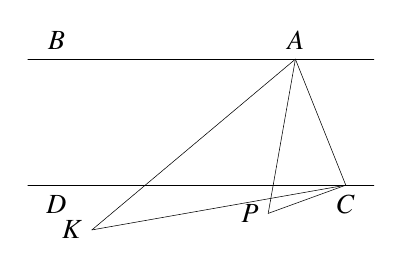
\begin{tikzpicture}[
        scale=0.8,
        decoration={
          markings,
          mark=at position 3cm with {\arrow[scale=2]{>}};
        }]
        % 初始化
        \tkzInit[xmin=-0.25,xmax=5.25, ymin=-1.00,ymax=2.5] \tkzClip
        % 定义坐标点
        \tkzDefPoints{0/0/E, 5/0/F, 0/2/R, 5/2/S}
        % 绘制两条平行线
        \tkzDrawLines(E,F R,S)
        % 定义A、B、C、D坐标
        \tkzDefPoints{0.2/0/D, 4.8/0/C, 0.2/2/B, 4.0/2/A}
        % 绘制各线段
        \tkzDrawSegments(A,C)
        % 标记符号
        \tkzLabelPoints[above](A,B)
        \tkzLabelPoints[below](D,C)
        % 定义A出发-120度的线
        \tkzDefShiftPoint[A](-100:1){a}
        % 定义C出发110度的线
        \tkzDefShiftPoint[C](-160:1){c}
        % 求交点
        \tkzInterLL(A,a)(C,c) \tkzGetPoint{P}
        \tkzLabelPoints[left](P)
        % 绘制线段
        \tkzDrawSegments(A,P C,P)   
        % 绘制角平分线关系
        \tkzDefLine[bisector](B,A,P) \tkzGetPoint{a}
        \tkzDefLine[bisector](P,C,D) \tkzGetPoint{c}    
        % 求交点
        \tkzInterLL(A,a)(C,c) \tkzGetPoint{K}
        \tkzLabelPoints[left](K)
        % 绘制线段
        \tkzDrawSegments(A,K C,K)
      \end{tikzpicture}
    }{\caption{}\label{fig03}}
  \end{floatrow}
\end{figure}

\begin{proof}[\textbf{(1)解}]
  $\because AB \varparallel CD$

  $\therefore \angle BAC + \angle DCA = 180^\circ$

  又$\because \angle BAC = \angle BAP + \angle PAC$
  
  $\angle DCA = \angle ACP + \angle DCP$

  $\therefore \angle BAP + \angle PAC + \angle ACP + \angle DCP = 180^\circ$

  又$\because$三角形内角和$=180^\circ$
  
  $\therefore \angle APC + \angle PAC + \angle ACP = 180^\circ$

  从而可得:
  \begin{align*}
    \angle APC & = \angle BAP + \angle DCP \\
               & = 60^\circ + 20^\circ\\
               & = 80^\circ                 
  \end{align*}  
\end{proof}

\begin{proof}[\textbf{(2)解}]
  $\because AB \varparallel CD$

  $\therefore \angle BAC + \angle DCA = 180^\circ$

  又$\because \angle BAC = \angle BAP + \angle PAC$
  
  $\angle DCA = \angle ACP + \angle DCP$

  $\therefore \angle BAP + \angle PAC + \angle ACP + \angle DCP = 180^\circ$

  又$\because$三角形内角和$=180^\circ$
  
  $\therefore \angle APC + \angle PAC + \angle ACP = 180^\circ$

  $\therefore \angle APC = \angle BAP + \angle DCP$

  同理可得:
  $\therefore \angle AKC = \angle BAK + \angle DCK$
  
  又$\because K$是$\angle BAP$与$\angle DCP$的角平分线的交点

  从而可得:
  \begin{align*}
    \angle AKC & = \frac{1}{2}\angle BAP + \frac{1}{2}\angle DCP \\
               & = \frac{1}{2}\left(\angle BAP + \angle DCP\right) \\
               & = \frac{1}{2}\angle APC                 
  \end{align*}  
\end{proof}

\begin{proof}[\textbf{(3)解}]
  $\because AB \varparallel CD$

  $\therefore \angle BAC + \angle DCA = 180^\circ$

  又$\because \angle BAC = \angle BAP + \angle PAC$
  
  $\angle DCA = \angle ACP - \angle DCP$

  $\therefore \angle BAP + \angle PAC + \angle ACP - \angle DCP = 180^\circ$

  又$\because$三角形内角和$=180^\circ$
  
  $\therefore \angle APC + \angle PAC + \angle ACP = 180^\circ$

  $\therefore \angle APC = \angle BAP - \angle DCP$

  同理可得:
  $\therefore \angle AKC = \angle BAK - \angle DCK$
  
  又$\because K$是$\angle BAP$与$\angle DCP$的角平分线的交点

  从而可得:
  \begin{align*}
    \angle AKC & = \frac{1}{2}\angle BAP - \frac{1}{2}\angle DCP \\
               & = \frac{1}{2}\left(\angle BAP - \angle DCP\right) \\
               & = \frac{1}{2}\angle APC                 
  \end{align*}  
\end{proof}

        % Using \verb|align|
        
        % \begin{align*}
        %       \because \triangle \mathrm{ABC}   &= \triangle \mathrm{A^{'}B^{'}C^{'}}   \\
        %       \therefore\, \angle \mathrm{ABC}  &= \angle  \mathrm{A^{'}B^{'}C^{'}}     \\
        %       \angle \mathrm{ACB}               &= \angle \mathrm{A^{'}C^{'}B^{'}}      \\
        %       \angle \mathrm{BAC}               &= \angle \mathrm{B^{'}A^{'}C^{'} }
        % \end{align*}
        
        % Using \verb|alignat|
        % \begin{alignat*}{3}
        %       &\because   &\triangle \mathrm{ABC} &= \triangle \mathrm{A^{'}B^{'}C^{'}}   \\
        %       &\therefore &\angle \mathrm{ABC}    &= \angle \mathrm{A^{'}B^{'}C^{'}}      \\
        %       &           &\angle \mathrm{ACB}    &= \angle \mathrm{A^{'}C^{'}B^{'}}      \\
        %       &           &\angle \mathrm{BAC}    &= \angle \mathrm{B^{'}A^{'}C^{'} }
        %     \end{alignat*}

\newpage

      \begin{tikzpicture}[
        scale=1.5,
        decoration={
          markings,
          mark=at position 3cm with {\arrow[scale=2]{>}};
        }]
        % 初始化
        \tkzInit[xmin=-0.25,xmax=3.25, ymin=-1.00,ymax=2.5] \tkzClip
        % 定义坐标点
        \tkzDefPoints{0/0/E, 3/0/F, 0/2/R, 3/2/S}
        % 绘制两条平行线
        \tkzDrawLines(E,F R,S)
        % 定义A、B、C、D坐标
        \tkzDefPoints{0.2/0/D, 2.8/0/C, 0.2/2/B, 2.0/2/A}
        % 绘制各线段
        \tkzDrawSegments(A,C)
        % 标记符号
        \tkzLabelPoints[above](A,B)
        \tkzLabelPoints[below](D,C)
        % 定义A出发-120度的线
        \tkzDefShiftPoint[A](-120:1){a}
        % 定义C出发110度的线
        \tkzDefShiftPoint[C](160:1){c}
        % 求交点
        \tkzInterLL(A,a)(C,c) \tkzGetPoint{P}
        \tkzLabelPoints[above left](P)
        %\tkzShowLine[parallel=through P](E,F)
        \tkzDefLine[parallel = through P](E,F) \tkzGetPoint{p}        
        \tkzDrawLines[color = red,add=.6 and .6,dashed](P,p)
        % 求交点
        \tkzInterLL(P,p)(A,C) \tkzGetPoint{Q}
        \tkzLabelPoints[above right](Q)
        % 绘制线段
        \tkzDrawSegments(A,P C,P)   
        \tkzMarkAngle[fill=red,size=0.5](P,C,D)
        \tkzLabelAngle[pos=1.2](P,C,D){$20^\circ$}
        \tkzMarkAngle[fill=blue,size=0.5](B,A,P)
        \tkzLabelAngle[pos=-0.9](P,A,B){$60^\circ$}
      \end{tikzpicture}
\vspace{-8ex}   
\begin{proof}[\textbf{(1)解}]
  过$P$点作辅助线$PQ$,并且使$PQ \varparallel CD$

  $\because AB \varparallel CD$

  $\therefore \angle APQ = \angle BAP$,并且$\angle CPQ = \angle DCP$

  从而可得:
  \begin{align*}
    \angle APC & = \angle APQ + \angle CPQ \\
               & = \angle BAP + \angle DCP \\
               & = 60^\circ + 20^\circ\\
               & = 80^\circ                 
  \end{align*}  
\end{proof}
  
\end{document}

%%% Local Variables:
%%% mode: latex
%%% TeX-master: t
%%% End:
